% \documentclass[a4paper,12pt]{report}   
\documentclass[a4paper,14pt]{extreport}
\usepackage{geometry}
% Margins and page layout %
% \usepackage[a4paper,left=30mm,right=20mm,top=20mm,bottom=20mm]{geometry}

% \usepackage{fancyhdr}
% \pagestyle{fancy} %Page Header

\usepackage{fancyref} %fun reference e.g.: /ref{subsec:phase2}

% Tiyle/Author %
\usepackage{authblk}

% Fonts %
\usepackage[utf8]{inputenc}
\usepackage[english]{babel}

% Paragraphs %
\usepackage{indentfirst}

% Bibliography %
%\usepackage{cite}
\usepackage[sort]{natbib}
\usepackage{url} % Use it later

% Hyperlinks %
\usepackage[linktocpage=true,plainpages=false,pdfpagelabels=false]{hyperref}
\usepackage{xcolor}

% Graphics %
\usepackage{graphicx}

% For including Source code %
\usepackage{listings} 

% \usepackage{lastpage} %Try it

% Numbering elements like, 
% Lemma 1. Unit Test-.., Theorema 3. Sth - .. 
\usepackage{amsthm} %

% Mathematics
\usepackage{amsmath}

% Custom list of 'element's
% \usepackage{tocloft}

% Using underscore sign %
\usepackage{underscore}

% Contents %
\usepackage{tocloft}

\usepackage{fixltx2e}
% for displaying fun algorithms
\usepackage[tworuled]{algorithm2e}

\usepackage{times} 
% \setmainfont{Times New Roman} 

% \geometry{a4paper,top=2.5cm,bottom=2.5cm,left=2.5cm,right=2.5cm}

 	%Load packages
%%% Page Layout %%%
\geometry{a4paper,left=30mm,right=20mm,top=20mm,bottom=20mm}

%%% Fonts %%%
% \renewcommand{\rmdefault}{ftm} % Times New Roman
\fontencoding{T1}
\fontfamily{garamond}
%   \fontseries{m}
%   \fontshape{it}
\fontsize{14}{16}
%   \selectfont

%%% Alignment and transfers %%%
\sloppy					% Get rid of the overflow
\clubpenalty=10000		% Forbid a page break after the first line of a paragraph
\widowpenalty=10000		% Forbid a page break after the last line of the paragraph

%%% Bibliography %%%
\bibliographystyle{unsrt}

%%% Images %%%
\graphicspath{{images/}} % ref to images dir

%%% Color of hyperlinks %%%
\definecolor{dark-red}{rgb}{0.4,0.15,0.15}
\definecolor{dark-blue}{rgb}{0.15,0.15,0.4}
\definecolor{medium-blue}{rgb}{0,0,0.5}
\hypersetup{
    colorlinks, linkcolor={dark-blue},
    citecolor={dark-blue}, urlcolor={medium-blue}
}

% Name style for List of Examples and impl %
\newcommand{\listexamplename}{List of Examples}
\newlistof{example}{exp}{\listexamplename}
\newcommand{\example}[1]{%
	\refstepcounter{example}
	\par\noindent\textbf{Example \theexample. } #1
	\addcontentsline{exp}{example}
	{\protect\numberline{
		\textbf{\thechapter.\theexample}}  #1
	}\par
}

% \etocsetstyle{chapter}
% {\parindent 0pt\leftskip 0pt\relex \rightskip .75cm \nobreak \etocskipfirstprefix}
% {\pagebreak[3]\bigskip}
% {\bfseries\large Chapter \etocnumber{} \etocname\par}
% {}

\renewcommand{\cftchappresnum}{Chapter }
\cftsetindents{chapter}{0em}{5em}
\cftsetindents{section}{0em}{5em}

% \setlength{\cftchapnumwidth}{2.6cm}
% \renewcommand{\cftchapfont}{\scshape}
% \renewcommand{\cftchappresnum}{\chaptername\ }
\renewcommand{\cftchapaftersnum}{.}{\cftchapaftersnumb}
% \renewcommand%{\newline}
\renewcommand{\cftchapdotsep}{\cftdotsep} % dots between chapter and number

\renewcommand*{\thesection}{\arabic{section}} % style section numbering. (1 sechtion_name)

%Definition
\newtheorem{defn}{Definition}

% no number starting from subsections downwards either in the document and in the TOC
\setcounter{secnumdepth}{1}
\setcounter{tocdepth}{1} 

% line spacing
\linespread{1.5}


% \titleformat{\chapter}[display]% OLD
%     {\normalfont\huge\bfseries}{\chaptertitlename\ \thechapter}{20pt}{\Huge}% OLD
% \titlespacing*{\chapter}{0pt}{50pt}{40pt}% OLD
\titleformat{\chapter}[display]% NEW
    {\normalsize\bfseries\centering}{\chaptertitlename\ \thechapter}{5pt}{\normalsize}% NEW
\titlespacing*{\chapter}{0pt}{30pt}{20pt}% NEW

\titleformat*{\section}{\normalsize\bfseries}
\titleformat*{\subsection}{\normalsize\bfseries}
\titleformat*{\subsubsection}{\normalsize\bfseries}

% listings styles
\lstset{language=java,
           basicstyle=\footnotesize,
           breaklines=true,
           keywordstyle=\color{blue}\ttfamily,
           stringstyle=\color{red}\ttfamily,
           commentstyle=\color{green}\ttfamily
          }
% \newcommand{\listdefinitionname}{List of Definition}
% \newlistof{definition}{defi}{\listdefinitionname}
% \newcommand{\definition}[1]{%
% 	\refstepcounter{definition}
% 	\par{Definition \thedefinition. #1}
% 	\addcontentsline{defi}{definition}
% 	{\protect\numberline{
% 		\thechapter.\thedefinition}#1
% 	}\par
% } 

%%% Contents %%%
% \renewcommand{\cftchapdotsep}{\cftdotsep} 		%User styles
 
\title{Filogenetik  ma'lumotlarni tahlil qilish prosedurasini ishlab chiqish}
\author{Javlon Eraliyev Rustambekovich}
% Johannes Kepler University, Linz, Austria %

\begin{document} 
\pagenumbering{gobble}

\thispagestyle{empty}

\begin{center}
\MakeUppercase{\bf{The State Committee for Communication, 
Informatization and Telecommunication Technologies of the 
Republic of Uzbekistan}}
\par
\MakeUppercase{\bf{Tashkent university of information technologies}}
\end{center}

\vspace{20mm}

\begin{flushright}
\textit{Manuscript rights}\par
UDC 004.4'2:61
\end{flushright}

\vspace{20mm}

\begin{center}
\MakeUppercase{Eraliyev Javlon Rustambekovich}
\vspace{10mm}

%��������� ���������������� ������ �� ����:\par
\textbf{Development of phylogenetic data analysis system}\par

\vspace{10mm}

5A330201 - Computer systems and software

\vspace{30mm}

In partial fulfilment of\par
the requirements for the degree of\par 
Masters of Sciences

\vspace{10mm}

\begin{flushright}
Research supervisor:\par
M Hudayberdiyev\par
\end{flushright}

\end{center}
% \vfill % fill until bottom
\begin{center}
Tashkent - 2014
\end{center}

\newpage 


% \setcounter{page}{1} 	% reset page counter
% \pagenumbering{roman}	% numerate pages as I,II,III,..

% \chapter*{Abstract} 
% \addcontentsline{toc}{chapter}{\numberline{}Abstract} %include page number to ToC%
Bioinformatics has gained increased usage and attention the last years.
In particulary, one of the main part of it philogenetics. 
But, if one wants to analize own research tests in this field, appropriate applications 
are still lagging behind.

This thesis brings Phylogenetics and Informatics together. 
It describes the implementation of a modern algorthms
into the Phylogenetic data analizing system. 

In particulary, algorithms of estimate calculations \cite{kamilov} and how they
differ from traditional algorithms discussed.

Aim is to provide a different approach for the 
construction of Phylogenetic Trees using different algorithms.\cite{juravlyov}

Both the general and unique features of the system discussed. Also, 
described new features in our analizing system, which were decided 
and added through an evaluation process.

Given examples how to use the analisis system.\par
% \textbf{
% For an MA thesis, the abstract should be between 100 and 250 words, depending on 
% departmental requirements. For the length of a PhD abstract, please consult departmental
% The abstract should normally include the following information: (1) a statement 
% of the problem the research sets out to resolve; (2) the methodology used; (3) the major 
% findings. Other information is optional unless required by the department.
% } 

\vspace{10mm}
% Filogenetik ma'lumotlarni tahlil qilish prosedurasini ishlab chiqish.\par
% Oxirgi yillarda bioinformatika sohasining ko'lami anchagina kengaydi va ommalashdi.
% Xususan, tirik organizmlarning rivojlanishini va o'zgarishlarini o'rganuvchi fan, 
% filogenetika, ham shularga ichiga kiradi. Xozirgi kunning informatika sohasidagi 
% yutuqlarga qaramasdan, filogentik ma'lumotlarni o'rganuvchi izlanuvchilar uchun 
% amaliy dasturiy ta'minotlar sezirarli orqada qolmoqda.

% Bu dissertatsiya ishida zamonaviy algoritmlar yordamida filogenetik ma'lumotlarni
% tahlil qilish usullari izohlangan. Xususan, baholash algoritmlari haqida va ularning 
% boshqa usullardan farqlari haqida so'z boradi.

% Maqsad, turli hil usullardan foydalanib filogenetik ma'lumotlarni tahlil qilish va 
% natijada filogenetik daraxtlar quradigan tizim ishlab chiqishdan iborat. 

% Tizimning asosiy va o'ziga hos imkoniyatlari ko'rsatib o'tilgan.

% Foydalanuvchilar uchun misollar bilan ko'rsatmalar keltirilgan.
\textbf{Uzbekcha}

Hozirda fan taraqqiyoti tadqiq qilinayotgan ob'ektlar yoki ob'ektlar
jamlanmasi tarkibi murakkabligining ortib borishi kuzatilmoqda. 
Ob'ektlar haqidagi axborotning oshib borishi, ushbu axborotni saqlash 
va qayta ishlash uchun kompyuter vositalarining qo'llanilishi, amaliyotda 
to'planagan axborotlar tarkibiga yashiringan qonuniyatlarni aniqlash 
hamda ijobiy hal qilish masalalari yanada dolzarb bo'lib bormoqda. 
Ma'lumotlarni saqlash uchun ma'lumotlar bazasini (MB) yaratish ehtiyoji 
tug'ilib, uning vositasida to'plangan ma'lumotlarga samarali ishlov berish 
yondashuvlari va tizimlarini ishlab chiqish zarur. Bunday mexanizmli 
vositalarni ishlab chiqishda so'ngi vaqtlarda shiddat bilan rivojlanayotgan 
ma'lumotlarni intellektual tahlili usullaridan unumli foydalanish 
maqsadga muvofiq. Ma'lumki, ma'lumotlarni intellektual tahlilining 
asosiy masalalari kassifikatsiya, regressiya, bashoratlash, assotsiativ 
qoidalarni qidirish, klasterizatsiya masalalarini qamrab oladi. 

Biologik tasniflar va ma'lumotlar bazasi yuzlab, minglab va undan 
ham ko'p turli xil darajadagi yuzlab belgilarga ega bo'lgan taksonlardan 
tashkil topadi. Kompyuter aniqlagichlari uchun bunday katta hajmdagi MB 
asosida tasniflashni amalga oshirish juda muhim hisoblanib, bunda qaror 
qabul qilish uchun eng maqbul muqobilni olish talab etiladi.
 
O'simliklar, xayvonlar va zamburug'lar aniqlagichlari 300 
yildan beri biolog olimlar 
tomonidan tadqiq qilib kelmoqda va ularning tuzilish usullari muhokama 
qilinmoqda, ularning biologik tasniflarini sistematik kalitlar 
yordamida dastlabki avtomatizatsiyalash o'tgan asrlardagi hisoblash 
texnikasi yordamida amalga oshirilgan. Tasniflash juda ko'pgina biologik 
tadqiqotlar jarayonida soha olimlarining amaliyotida muhim ahamiyat kasb 
etadi.

O'zbekiston biolog olimlari uchun ham yuqoridagi kabi muammolar vujudga 
kelmoqda. Shuning uchun, tahlillardan kelib 
chiqib qisman pretsendentlikka asoslangan timsollarni 
aniqlash algoritmi asosida biologik tizimlarni tasniflash va tadqiq qilish 
tizimini tashkil etish tadqiqotning dolzarbligini belgilaydi.

\newpage


% \chapter*{Preface}
\addcontentsline{toc}{chapter}{\numberline{}Preface} %include page number to ToC
This report represents the work done in my master's thesis (Master of
Science) in Computer Science at the Department of The Faculty of 
Engineering and Natural Sciences (TNF) at the Johannes Kepler University (JKU) 
Linz, Austria. My supervisors have been DI Dr. Professor Windsteiger Wolfgang 
at Research Institute for Symbolic Computation (RISC) which is an institute of 
JKU, who has patiently endured questions and provided both encouragement and criticism.
	

Many thanks also to Prof. Dr.Dr.h.c.mult. Buchberger Bruno at RISC, who is the 
head of Softwarepark Hagenberg, for acceptance to ISI-Program, for helps and 
for giving motivation for my future works. Who came up with idea of creating 
proving system Theorema.
\newpage
 
\tableofcontents

\newpage

% \listofexample
% \newpage

% \listofdefinition
% \newpage

% \textbf{1.3.6 List of Figures, Tables or Illustrations}
% If appropriate, a separate list of figures, tables, or illustrations should be included on a 
% separate page immediately following the table of contents.
% 
% \textbf{1.4.2 Glossary}
% A list of special technical words or acronyms may be necessary. This is particularly true if 
% the subject deals with a new area with a specialised vocabulary that the average reader in 
% the discipline might not be familiar with, such as the Internet. This list should come after the 
% appendices.
% 
% 
% When \cite{texbook} using numbers in the text, numbers up to one hundred should normally be written in 
% words, and if the first word of a sentence is a number it should be written in words. Numbers 
% above one hundred are usually written as numerals (101, 102). For precise guidance, students 
% should consult the style manual recommended by their \cite{primes} department.

\pagenumbering{arabic}	% numerate pages as 1,2,3,..
\setcounter{page}{7} 	% reset page counter

% Kirish
\chapter*{Introduction}
 \addcontentsline{toc}{chapter}{\numberline{}Introduction}
\begin{quote}
%Add abstract here
\end{quote}

Phylogenetic is the study of the evolutionary histories of living 
organisms, and represent the evolutionary divergences by finite 
directed (weighted) graphs, or directed (weighted) trees, known 
as \textit{phylogeny}. Based on molecular sequences, phylogenetic trees 
can be built to reconstruct the evolutionary tree of species involved. 
In particular, the representation derived from genes or protein 
sequences is known as \textit{gene phylogeny}, while the representation 
of the evolutionary path of the species are often referred as 
species \textit{phylogeny}. A gene phylogeny is, to some extend, a local desciption. 
It only describes the evolution of a particular gene or encoded protein, 
and this sequence could evolve much more or less differently than 
other genes in the genome, or it may have completely different 
evolutionary history from the rest of the genome due to horizontal 
gene transfers. Therefore, the evolution of a particular gene only 
provides a local picture, not necessarily reflect the \textit{global} 
evolutionary picture of the species. We can only hope that we could 
assemble the jigsaw puzzle pieces with a wide selection of gene 
family to give an overall assessment of the species evolution. 

While in general the topology in phylogenetic trees represents 
the relationships between the taxa, assigning scales to edges 
in the trees could provide extra information on the amount of 
evolution divergence as well as the time of the divergence. 
The phylogenetic trees with the scaled edges are called \textit{phylograms}, 
while the non-scaled phylogenetic trees are called \textit{cladograms}. 
Purely for the sake of computers data processing, some special 
formats were artificially created, such as Newick format. From 
biological point of view, the building of phylogenetic trees 
can be roughly divided into the following steps. 


\textbf{Choose molecular marker.}
In building molecular phylogenetic trees, either nucleotide 
or protein sequence data can be used, but the outcomes from 
the choice could be quite different. The rule of thumb is to 
select nucleotide sequences when some very closely related 
organisms are studied because they tend to evolve more rapidly 
than proteins; and to select protein sequence (or slowly evolving 
nucleotide sequences) when more widely divergent groups of 
organisms are studied.


\textbf{Perform sequence alignment.}
 The sequence alignment establishes positional correspondence 
 in evo- lution, and aligned positions are assumed to be 
 genealogically related. Though there have been numerous 
 so-called \textit{state-of-art} alignment programs available and 
 many times they do help, manual editing is often
 crucial in the quality of alignment, and yet there is 
 no firm or clearly defining rule on how to modify a 
 sequence alignment. 
 
 
 \textbf{Choose a model of evolution.}
  One quantitate measure of divergence between two 
  sequences is the number of substitutions in an alignment. 
  However, this measure can somehow be misleading in 
  representing the true evolution. Not only the nucleotide 
  may actually undergone several intermediate steps of 
  changes behind a single mutation in the sequence, but 
  also an observed identical nucleotide may hide parallel 
  mutations of both sequences. This is known as homoplasy. 
  The statistical models used to correct homoplasy are 
  called evolutioinary models. For constructing DNA 
  phylogenies, there have been Jukes-Cantor model and 
  Kimural model.
  
 
\textbf{Determine a tree building method.}
 There are basically two types of phylogenetic 
 methods, character based methods and distance 
 based methods. Character-based methods based on 
 discrete characters from molecular sequences from 
 individual taxa. The theory is that characters at 
 corresponding positions in a multiple sequence 
 alignment are homologous (this word has different 
 meaning in mathematics and is precisely defined for 
 sequences with differentials.) among the sequences 
 involved. On the other hand, distance-based methods is 
 based on the distance, the degrees of differences between 
 pairs of seqeuences. Such distance will be used to construct 
 the distance matrix between individual pairs of taxa. 
 The theory in this case is that all sequences involved 
 are homologous and the weighted directed tree will 
 satisfy the additive properties. There are two different 
 algorithms in distance based method, the cluster-based 
 and the optimality-based. The cluster-based method 
 algorithms build a phylogenetic tree based on a distance 
 matrix starting from the most similar sequence pairs. 
 The algorithms of cluster-bsed include unweighted pair 
 group method using arithmetic average (UPGMA) and 
 neighbor joining (NJ). The optimality-based method 
 algorithms compare numerous different tree topologies 
 and select the one which is believed to best fit between 
 computed distances in the trees and the desired 
 evolutionary distances which often referred as actual 
 evolutionary distances. Algorithms of optimality based 
 include Fitch-Margoliash and minimum evolution. 
% \section*{}
\subsection*{Motivation}
The root of the problem lies in the lack of a certain mechanism 
for analyzing phylogenetic sequences. This makes it possible to 
analyze and build phylogenetic trees from given data. The problem 
is to optimize constructing large trees using 
algorithms of estimate calculations.

The aim is to find an optimal solution in a set of candidate solutions. 
There are other types of problems besides optimisation and decision problems. 
This dissertation will deal with optimisation problems.

Problems are not only categorised on the basis of the types of 
answer they seek, but also on the basis of how complex it is to 
compute the answers. For some problems, there is no algorithm 
giving always the correct answer. For most of the problems 
encountered in practice, however, the complexity of their 
solution is measured in terms of the amount of computational 
resources (typically time and memory space) that algorithms need 
in order to compute the correct output.

\subsection*{Research object}
Phylogeny, phylogenetic tree and phylogenetic sequences.

\subsection*{Research subject}
Methods of phylogenetic analysis, phylogenetic analysis algorithms, 
phylogenetic analysis software are the object of research. 

\subsection*{Research question} 
%\addcontentsline{toc}{section}{\numberline{}Research question}

The following research questions were defined from given below 
background of the problem:

How can be used algorithms of estimate calculations in phylogeny 
analyzing systems?;

Can algorithms of estimate calculations improve efficiency of phylogeny 
analizing systems?;

\subsection*{Research goals} 

Learn and analyze phylogenetic analysis systems and softwares;

Find main characteristics and ways for improving phylogenetic analysis;

Define methods and concepts for phylogenetic data analysis;

Develop process for phylogenetic data analysis;

Integrate algorithms of estimate calculations into phylogenetics;	

Develop phylogenetic data analysis software; 

\subsection*{Research hypothesis}
Algorithms of estimate calculation are more efficient to 
reconstruct phylogenetic tree.

\subsection*{Existing researches}
There are many foregn researches and articles 
devoted to the phylogenetics.
Scientists use results of the researches in real 
world projects and analysis . For example, in biology, 
in medicine and etc.

Developed many programms such as PHYLIP, PAUP, MacClade, 
TREECON, Spectrum, TREEMAP, DNA Stacks, GeneDoc, Seq-Gen, 
Phylodendron, GeneTree, PASSML, BioEdit, MEGA, PAST, ClustalW and etc.

Found that developed products have many advantages and some 
disadvantages. Main disadvantages are related with efficiency. 
No product which uses algorithms of estimate calculations.

\subsection*{Researches methods}
Systematic analysis, cluster analysis, programming techniques and 
methods, modelling, benchmarking and comparative methods are used.

\subsection*{Theoretical and practical importance}
Developed software can be used by scientists in biology.
Implemented methods are more efficient for reconstructing
phylogenetic trees.

\subsection*{Benefit for the Science and contributions}
Analized pro and cons of available phylogenetic tree building systems;

Improved a process and methods of phylogenetic tree reconstructing;

Developed software using the process and the methods;

\subsection*{Content}
The Thesis includes introduction, 3 chapters, 
each chapter has a introduction and summary, 
conclusion, references and applications. 
Main part of the thesis wrote in 54 pages.
% Although the first section of each chapter gives an overview of
% its contents, below outlined the contents of each chapter in a more 
% concise way.

% In the first chapter, we will discuss definitions of 
% phylogeny, trees, gene, gene sequence and 
% algorithms of estimate calculations. We will analyze 
% major concepts of phylogeny.
% 
% In the second chapter, we will discuss state of art and how the 
% algorithms of estimate calculations can be used to solve problem. Also, types of phylogenetic 
% tree reconstruction methods and approaches to tree 
% building are discussed. Comparisons between methods are given.
% 
% In the third chapter, the overall section, 
% of this document gives an overview of the functionality 
% of the product. It describes the informal requirements 
% and is used to establish a context for the technical 
% requirements specification in the next chapter.
% Requirements Specification section, of this document is written 
% primarily for the developers and describes in technical 
% terms the details of the functionality of the product. 
% Both sections of the document describe the same software 
% product in its entirety, but are intended for different 
% audiences and thus use different language. 

 

% BOB I
\chapter{General concept and analysis of existing 
methods for the analysis of phylogenetic data}

\newtheorem{defi}{Definition} % Start new Definetion numbering

\section{General concepts of phylogeny}
\subsection{Overview}

The branching pattern of ancestor/descendant relationships among species or
their parts (e.g., genes) is a phylogeny. Researchers attempt to estimate these 
historical relationships by examining character evolution using a tree - a mathematical
structure used to model the actual evolutionary history of species or their parts.
These inferred trees (historical branching relationships) can be represented as 
cladograms, where branch lengths are arbitrary and only the branching order is significant,
or as phylograms, where the branch lengths are proportional to the amount of evolutionary 
change along the branch.

Phylogenies were historically used to classify organisms into natural evolutionary
groups based on these ancestor/descendant relationships. Indeed, great effort is
currently being spent on estimating the Tree of Life to quantify the biodiversity of
our planet. However, phylogenies have also spread in use as the utility of the
evolutionary framework for numerous other disciplines becomes increasingly obvious. 
For example, phylogenies are now being extensively used in the biomedical sciences 
including developmental biology, genomic biology, infectious disease, virology,
and human genetics \cite{jumpstarting}.

\subsection{Phylogenetic Tree}
Since this thesis is about phylogenetic trees, it is therefore 
appropriate to start by defining a tree \cite{alkim}. 
Trees can be classified as unrooted or rooted phylogenetic trees. An 
unrooted phylogenetic tree or just unrooted tree is an acyclic connected 
graph having no internal vertices of degree two and every leaf having 
different label. The leaves are vertices of degree one \ref{img:sample1}.

\begin{figure}[!htbp]
  \center
  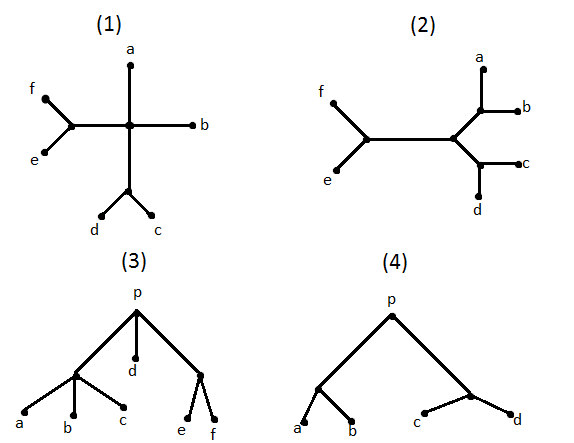
\includegraphics[width=0.5\textwidth]{tree1}
  \caption[w]{Four examples of phylogenetic trees. (1) and (2) are unrooted. (3) and 
(4) are rooted. (2) and (4) are binary. } 
  \label{img:sample1}  
\end{figure}

A rooted tree on tree, on the other hand, is similar to an unrooted 
tree, except it has one internal vertex of degree two, which is called the 
root. The internal vertices of unrooted/rooted (except the root) trees can 
have degree three or greater. For example a binary phylogenetic tree, is a 
tree having all internal vertices of degree three. Again the only exception is 
the root, which has degree two \ref{img:sample2}. In a fully resolved binary 
phylogenetic tree with n leaf nodes there are n-1 internal nodes. 

\begin{figure}[!htbp] 
  \center
  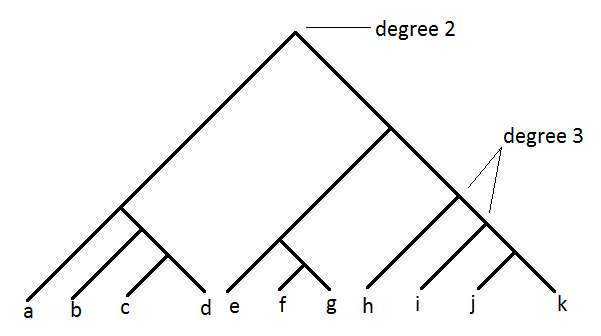
\includegraphics[width=0.5\textwidth]{tree2}
  \caption[w]{In a binary tree each internal node has degree three with the 
exception of the root which has degree two.} 
  \label{img:sample2}  
\end{figure}

The leaves of the tree represent species. For example let L(T) be the 
set of leaves for tree T. If T the set of trees, then we can say that L(T) is the 
union of the leaf sets of the trees in T. 

The vertices adjacent to a vertex that are descendants of the vertex 
are called the children of the vertex, and the adjacent vertex that is an 
ancestor is called the parent of that vertex. Sometimes the internal 
vertices of a phylogenetic tree are labelled (section Nested Taxa). 

Rooted phylogenetic trees can be displayed with a vertical axis 
representing the time each branching point occurred. These diagrams are 
called dendograms \ref{img:sample3}. 

\begin{figure}[!htbp] 
  \center
  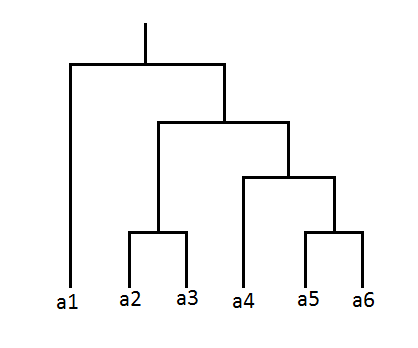
\includegraphics[width=0.5\textwidth]{tree3}
  \caption[w]{An example of dendogram.} 
  \label{img:sample3}  
\end{figure}

Let T be a rooted tree and choose a vertex v in T. If we remove the 
edge between v and the parent of v, say p, we get two connected 
subgraphs. Then let v be the root of the subgraphs containing v, then this 
is called the subtree of T rooted at v. Briefly a subtree T' is a tree whose 
vertices and edges form the subsets of the vertices and edges of a given 
tree T. An example of a subtree is shown in \ref{img:sample4}.

\begin{figure}[!htbp] 
  \center
  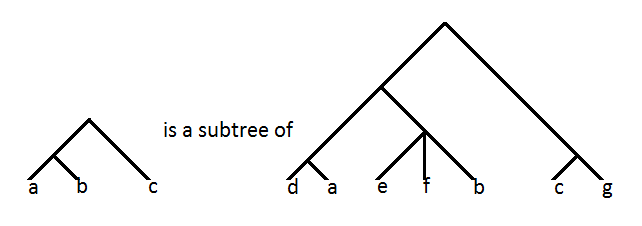
\includegraphics{tree4}
  \caption[w]{Example of a subtree.} 
  \label{img:sample4}  
\end{figure} 

For every three leaves a, b, c there are four possible rooted trees 
with leaf set a, b, c.  

The binary rooted trees on three leaves are called rooted triples and 
((ab)c) (or ab|c) denotes the rooted triple with a pair of leaves a, b 
connected to a third leaf c via the root (\ref{img:sample5}). For a rooted triple 
((ab)c) to fit a rooted tree T, the path from a to b does not share any 
vertices with the path from c to the root. Briefly a rooted triple is a tree 
with three leaves and two internal vertices. 

\begin{figure}[!htbp] 
  \center
  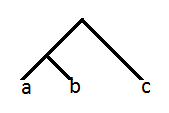
\includegraphics{tree5}
  \caption[w]{ A binary rooted triple ((ab)c).} 
  \label{img:sample5}  
\end{figure} 

Non-binary rooted trees with three leaves are called fan triples. We 
call a fan with k leaves a k-fan. 

% Also it has many useful features such as making presentations, 
% importing from most popular file formats as well as exporting 
% to these formats.

\section{Using Algorithms of Estimate Calculations for building distance matrix}
\subsection{Overview \cite{kamilov, juravlyov}} Most of the advanced data processing and analysis technologies 
designed for solving domain-specific problems employ the automation and 
optimization techniques of decision-making based on 'real' information. 
The methods of mathematical theory of pattern recognition play an important role here. 
To carry out image recognition, we need an image representation that 
corresponds to the requirements of the efficient recognition algorithm chosen 
for the task. A vast majority of the efficient image recognition algorithms 
only work with image descriptions or models. To completely use the information 
contained in images, it is necessary to overcome the principal discrepancy between 
the nature of images and the data-extraction techniques based on symbol models of 
images. Thus, there is a practical need for an efficient recognition algorithm that 
directly deals with images and their fragments. More-over, the algorithm should 
provide the possibility of posing and solving the problem of choosing the best
recognition algorithm. This class of algorithms - algorithms of estimate calculations 
based on 2D information - was defined by I. Gurevich as a special type of 
the classical model of the recognition algorithms based on estimate calculations 
(AEC) introduced by Yu. Zhuravlev. Generally, the AEC model can cope with the spatial 
(2D) image structure. In this work, we find these formulas more efficient to reconstruct
phylogenetic tree.

\subsection{Overview}

% Most of the current data technologies for information processing and analysis designed 
% to solve domain-specific content-driven problems employ the automation and optimization 
% techniques of operative decision-making based on 'real' (incomplete, indirect, heterogeneous,
% inconsistent, erroneous, etc.) information. These information technologies are widely 
% used in medical and technical diagnoses, nondestructive testing, ecological monitoring,
% natural disaster and emergency forecasting (like technogenic catastrophes, earthquakes, 
% fioods, forest fires), informa- tion and copyright protection, security systems, 
% scientific research automation, smart weapons, remote earth sensing, criminal law, 
% and control. The methods of mathematical theory of pattern recognition are the basic 
% tools for solving all of these problems. In most cases, when initial data are completely 
% or partly represented as images, it is necessary to use the methods of analysis and 
% estimation of information represented by images. 

The procedures of transforming the initial data in the form 
convenient for recognition should yield a mathematical model of an image. 
This model should refiect the inner structure and content of the image as an 
outcome of operations that construct the image from the subimages and other 
objects of simpler nature, i.e., from the primitives and objects extracted in the 
image at different stages of processing. During image recognition, one should use 
information refiecting the way of pattern formation, i.e., of the image as a whole, 
and of the objects presented in the image.  

Three types of information characterize an image: (i) identifiable objects with a 
well-defined structure; (ii) identifiable objects with an ill-defined structure; 
and (iii) nonidentifiable objects. To allow for an image structure means to extract 
subimages (objects) in an image, to define the possible elementary level for them, 
and to define the relations between these objects and elements. As a result, 
the hierarchical structural information of an image may be explicitly presented and 
utilized. An image is described by a system of objects, each object is described by 
simpler objects, etc. The structural information can be introduced into recognition 
process in two ways. 

First, according to classical pattern recognition theory, 
we can use the list of features as a main formalization principle and 

(a) two types of features are introduced in the description;
they refiect a two-dimensional character of the object to be recognized: 

-characteristics which refiect the properties of some local image fragment 
(the distribution of pixel values in this fragment, the presence or 
absence of a certain geometrical object in this fragment, the type of 
the object's shape, etc.); 

-characteristics of relations of separate objects and features; 

(b) the weights are assigned to the features, which indicate the degree 
of their importance for image description; 

(c) separate features are combined into a system of features and treated 
as a single feature. 

\subsection{General characterustics of the AEC class}

The model of algorithms based on calculation of the estimates 
(AEC) was successfully used for solving many problems of pattern 
recognition. The model describes the structure of recognition 
algorithm and parameters necessary for choosing particular 
algorithm in the model. In the framework of a model, the algorithms 
differ by their parameters and, therefore, by the way of their 
classification of the given objects. The results of applying the 
algorithm of a model to the test sample show the adequacy of this 
algorithm to the problem at hand. Thus, all of the algorithms 
of a given model can be supplied with a quality functional. 

The choice and/or synthesis of the algorithm, extreme according 
to the quality functional, presents the main problem in implementing 
AEC in practice. This problem is closely connected to the reduction 
of the computational complexity of AEC. The algorithms of acceptable 
computational complexity are based on efficient formulas which model 
the algorithm`s performance; these are formulas for calculating 
proximity estimates of objects under recognition and precedents. 
The complexity of formulas for estimate calculations substantially 
depends on the AEC parameters, such as the system of support 
sets and the type of proximity function. A recognition algorithm 
uses a system of support sets as a system of feature subsets 
for matching object descriptions. A proximity function defines 
whether the matched objects are 'close'. 
% 
% By now, the most comprehensive study concerned the problems 
% of deriving efficient formulas for AEC in the case where all 
% available objects are described by the one-dimensional feature 
% vectors and the support sets encode the parts of these one-dimensional 
% descriptions. This problem was solved for the main subclasses of AEC in.
% 
% When the efficient formulas for estimate calculations are constructed, 
% the optimal (for the given model) algorithm can be chosen by 
% one of the classical optimi- zation techniques or by modifying 
% these techniques. A lot of research was devoted to this problem.
  
Although the efficient formulas are constructed almost for every 
AEC model of practical interest, the problem of constructing such 
formulas in the case where the objects are images, object 
descriptions are 2D matrices, and support sets are spatial (2D) 
objects still needs to be solved. As was noted above, the AEC 
class was specialized to operate with 2D object descriptions 
called a class of algorithms of estimate calculation from 
two-dimensional information (2D-AEC). Note that, by now, 
the efficient formulas are con- structed for one 2D-AEC subclass 
only: for a subclass with a square as a generative element of the 
system of support sets.

Here, we propose the method for constructing the efficient algorithms 
for the 2D-AEC subclass with two-dimensional support sets generated 
by a rectangle. The idea underlying this procedure consists in 
transforming the rectangle with the sides  $R_1*R_2$  into 
the unit square by compressing the plane along the one side  $R_1$  
times and along the other  $R_2$  times. 

Let us recall the basic objects and properties of the AEC model 
Generally, a recognition algo- rithm contains a recognizing operator and a 
decision rule. In AEC, a recognizing operator converts a standard 
description of object $S$ , subject to recognition into a 
set of numerical estimates $(\Gamma_1(S),\Gamma_2(S),\ldots,\Gamma_l(S))$,
where $l$ is a number of clases.  A decision rule helps us to 
construct the information vector $(\alpha_1,\alpha_2,\ldots,\alpha_l)$,
$a_j\in\{0,1,\Delta\}$, from this set.  Here, $\alpha_j  = 0$ if an algorithm does not
assign object  $S$ to $j$th class;  and  $\alpha_j  =  \Delta$ 
if an algorithm cannot classify object  $S$ . To define a recognizing operator, 
it is necessary to assign a system of support sets, proximity function, 
feature weights, and precedent weights. Let us consider these parameters in detail.  

1. System of support sets. 

A system of support sets is a totality of nonempty subsets of the feature set  
$N  = \{1,2,\ldots,n\};$ the object is described by the values of these features. 
A system of support sets is denoted by  $\Omega_A$. 
Below, we list the examples of support sets.

1.1. $\Omega_A  = 2^N;$ i.e., a system of support sets is a class of all (nonempty) 
subsets of feature set  $N$.
 
1.2.  $\Omega_A=\{\Omega|\Omega\subseteq N,|\Omega|=k\}$, where  $k$  is an integer and $1\leq k\leq n;$ 
i.e., a system of support sets consists of all of the subsets of the set  $N$  which have 
a predefined power  k , e.g.,  $\Omega_A={{1},{2},\ldots,{n}}$ for  $k=1$ and $\Omega_A=\{N\}$ for  $k=n$. 
The following relation connects the systems of support sets of 1.1 and 1.2:

$$
2^N=\bigcup_{k=1}^n\{\Omega | \Omega \subseteq N, | \Omega | = k\}.
$$

1.3. $\Omega_A=\{\Omega|\Omega\subseteq N,|\Omega|\leq k\}$, where  $k$  is an integer
and $1\leq k\leq n;$ i.e.,  $\Omega_A$ consists of all of the subsets of the
set $N$ which have a power no more than the predefined one. 

1.4. $\Omega_A=\{\Omega|\Omega\subseteq N,|\Omega|\subseteq \{k_1,k_2,\ldots,k_u\}\}$, where 
$k_1,k_2,\ldots,k_u$  are integers and $1\leq k_i \leq n, i=\bar{1,n}$. 

Any support set $\Omega$ 
can be encoded by the binary vector $\tilde{\omega}$ of the length $n$ in the following way: 
the ith coordinate $\tilde{\omega}$ is equal to one if and only if the $i$th feature is contained 
in $\Omega$. The thus-constructed $\tilde{\omega}$ vector is called a characteristic vector 
of the support set $\Omega$. It is obvious that a set $\Omega$ and its characteristic 
vector $\tilde{\omega}$ are connected by a one-to-one correspondence.

Sometimes, it is convenient to consider a system of support sets as a set of characteristic 
vectors that encode the support sets of the algorithm. In those cases, we consider $\Omega_A$ 
to be a set of vertices $\{\tilde{\omega}\}$ of $n$-dimensional Boolean cube $E^n$. 

As usual, we denote the norm (weight) of the binary vector $\|\{\tilde{\omega}\}\|$ equal to 
the number of its unitary coordinates by $\{\tilde{\omega}\}$. The set of all binary vectors 
of the weight $k$ is called the $k$th layer of the Boolean cube and denoted by $E_n^k$.

We call the Boolean function $f_A(\tilde{\omega})$ a characteristic function of the system of support 
sets $\Omega_A$ if $f_A(\tilde{\omega})=1\Leftrightarrow \in \Omega_A$. Obviously, a system of support 
sets of the algorithm is unambiguously described by its characteristic function. 

The characteristic function of a system of support sets of (1.1)-type vanishes only if all its 
variables vanish.

For a system of support sets of (1.2)-type, the characteristic function is 
equal to unity in the whole layer of Boolean cube and only there.

For a system of support sets of (1.3)-type, the characteristic function is equal to 
unity in the whole first, second, \ldots, $k$th layers of Boolean cube and only there.   

2. Proximity function.

Let $I(S) = (a_1, a_2, \ldots, a_n)$ be a standard (feature) description of 
object $S, \Omega = \{i_1, i_2,\ldots, i_k\}$, and let  be a characteristic 
vector $\Omega$. We denote a subdescription of the object $S$ represented in 
the form $(a_{i_1}, a_{i_2} ,\ldots,a_{i_k})$ by the symbols 
$\tilde{\omega} I(S)$ or $\tilde{\omega}(S)$.

The proximity function $B_{\tilde{\omega}}(S, S')$ depends on $\tilde{\omega}$-subdescriptions 
of objects $S, S'$ and takes two values: 0 if the objects are not close and 1 otherwise. 

Most often, the following proximity functions are considered:

2.1
\begin{equation}
B_{\tilde{\omega}}(S, S') = \left\{ 
  \begin{array}{l l}
    1, \tilde{\omega}S = \tilde{\omega}S' \\
    0, \tilde{\omega}S \neq \tilde{\omega}S'
  \end{array} \right.
\end{equation}

2.2. Let the metric (or semimetric) $\rho_i(x, y), i = \bar{1,n}$, be defined on the 
range of definition of the $i$th feature. 
Let $\tilde{\omega}S=(a_{i_1}, a_{i_2}, \ldots, a_{i_k}), \tilde{\omega}S' = (b_{i_1}, b_{i_1}, \ldots, b_{i_1})$,
and the quantities $\varepsilon_i \geq 0, i = \bar{1, n}, \varepsilon \geq 0$, where $\varepsilon$ 
is integer, be set. Consider a system of inequalities
\begin{equation}
	\rho_{i_1}(a_{i_1}, b_{i_1}) \leq \varepsilon_{i_1},
	\rho_{i_2}(a_{i_2}, b_{i_2}) \leq \varepsilon_{i_2},
	\ldots,
	\rho_{i_k}(a_{i_k}, b_{i_k}) \leq \varepsilon_{i_k}	
\end{equation}
and denote the number of unsatisfied inequalities in this system by $\gamma$. Then,
\begin{equation}
B_{\tilde{\omega}}(S,S') = \left\{ 
  \begin{array}{l l}
    1, \gamma \leq \varepsilon \\
    0, \gamma > \varepsilon
  \end{array} \right.
\end{equation}

The parameters of this function are the vector 
$\varepsilon = (\varepsilon_1, \varepsilon_2, \ldots, \varepsilon_n)$ 
and the quantity $\varepsilon$ (maximally admissible number of unsatisfied 
inequalities in system (1.2)). If $\varepsilon_i = 0, i = \bar{1,n}$, and $\varepsilon = 0$, this 
proximity function is identically equal to the proximity 
function determined in 2.1.

2.3.  If in the conditions of the previous point, we set two 
integers $\varepsilon^1$ and $\varepsilon^2$ ($\varepsilon^1$, $\varepsilon^2$ $\geq$ 0) instead 
of $\varepsilon$, then

\begin{equation}
B_{\tilde{\omega}}(S, S') = \left\{ 
  \begin{array}{l l}
    1, \|\{\tilde{\omega}\}\| - \gamma \geq \varepsilon^1,\gamma \leq \varepsilon^2 \\
    0, \gamma > \text{otherwise}
  \end{array} \right.
\end{equation}

Vector $\varepsilon = (\varepsilon_1, \varepsilon_2, \ldots , \varepsilon_n)$ and 
quantities $\varepsilon^1$ and $\varepsilon^2$ (minimal accessible 
number of satisfied inequalities in system (1.2) and maximal accessible number 
of unsatisfied inequalities in system (1.2), respectively) are parameters of 
the function. For $\varepsilon^1 = 0$ and $\varepsilon^2 = \varepsilon$, we get the (2.2)-type proximity function.

Suppose once more that $I(S) = (a_1, a_2, \ldots, a_n)$,
$I(S') = (b_1, b_2, \ldots, b_n)$, the metric (or semimetric) $\rho_i(x, y)$
is defined in the range of definition of the ith feature, and the values $\varepsilon_i \geq 0, i = \bar{1, n}$ are set. 
The binary vector $\tilde{\delta} = \tilde{\delta}(S, S') = (\tilde{\delta}_1, \tilde{\delta}_2, \ldots, \tilde{\delta}_n)$ defined as follows: 

\begin{equation}
\delta_i = \left\{ 
  \begin{array}{l l}
    1, \rho_i(a_i,b_i) \leq \varepsilon_i \\
    0, \rho_i(a_i,b_i) > \varepsilon_i
  \end{array} \right.
\end{equation}

where $i = \bar{1,n}$, is called a characteristic vector of the proximity 
of objects $S$ and $S'$.

By using a characteristic vector of proximity, we can rewrite the expression for 
(2.2)-type proximity function as

\begin{equation}
B_{\tilde{\omega}}(S, S') = \left\{ 
  \begin{array}{l l}
    1, (\tilde{\delta'}, \tilde{\omega}) \leq \varepsilon \\
    0, (\tilde{\delta'}, \tilde{\omega}) > \varepsilon
  \end{array} \right.
\end{equation}

where $\tilde{\delta'}$ is a binary vector obtained by the coordinate-wise negation of vector 
$\tilde{\delta} $ and $(\alpha, \beta)$ is a scalar product of the vectors $\alpha$ and $\beta$ which is 
equal to the sum of their coordinatewise multiplications. 

In a similar way, for the (2.3)-type proximity function,

\begin{equation}
B_{\tilde{\omega}}(S, S') = \left\{ 
  \begin{array}{l l}
    1, (\tilde{\delta}, \tilde{\omega}) \geq \varepsilon^1, (\tilde{\delta'}, \tilde{\omega}) \geq \varepsilon^2 \\
    0, \text{otherwise}
  \end{array} \right.
\end{equation}

We can introduce vector $\tilde{\delta}(S, S')$ while ignoring the metric 
$\rho_i$ and quantities $\varepsilon_i$ in the following way:

\begin{equation}
\delta_i = \left\{ 
  \begin{array}{l l}
    1, a_i = b_i \\
    0, a_i \neq b_i
  \end{array} \right.
\end{equation}

In this case, the expression for the (2.1)-type proximity 
function can be rewritten in the following way:

\begin{equation}
B_{\tilde{\omega}}(S, S') = \left\{ 
  \begin{array}{l l}
    1, (\tilde{\delta}, \tilde{\omega}) = \|\tilde{\omega}\| \\
    0, (\tilde{\delta}, \tilde{\omega}) < \|\tilde{\omega}\|
  \end{array} \right.
\end{equation}

3. Feature weights. 

Feature weights are set by the vector 
$\textbf{p} = (p_1, p_2, \ldots, p_n), p_i > 0, i = \bar{1, n}$. 

Let ${i_1, i_2, \ldots, i_k}$ be a set of the indices of all unit 
coordinates of the characteristic vector $\tilde{\omega}$. The weight 
of the support set $\Omega$ with a characteristic vector $\tilde{\omega}$ 
is denoted by $p(\tilde{\omega});  p(\tilde{\omega}) = p_{i_1} + p_{i_2} + \ldots+ p_{i_k}$.

4. Precedent weights.

Precedent weights are defined by the vector 
$ \gamma = (\gamma_1, \gamma_2, \ldots, \gamma_{m})$, 
where $\gamma_q = \gamma(S_q)>0, q = \bar{1, m} $, and $m$ is a 
total number of precedents. This point concludes the list of 
the parameters of the recognition operator of AEC.

The estimate $\Gamma_j(S)$ of the object $S$ over the $j$th class 
is defined by the following formula:

\begin{equation}
\Gamma_i(S) = \frac{1}{K}\frac{1}{|W_j|}\sum_{S'\in W_j}\gamma(S')\sum_{\tilde{\omega}\in\Omega_A}p(\tilde{\omega})B_{\tilde{\omega}}(S, S'), j = \bar{1, l},
\end{equation}
where $K$ is a normalized coefficient and $W_j$ is a set of precedents of the $j$th class. 

Sometimes we use the formulas to assess an esti- mate $\Gamma_j(S)$ that differ from 
Eq. (1.10). In any case, however, the semantics of the initial formulas for $\Gamma_j$
is the same; i.e., over all of the support sets, the value of proximity function 
(and/or of its negation) is calculated for the given object $S$ and for each object $S'$ 
from the learning set. Each time, the weights of the features and the precedents 
are equally accounted of.

We finish the definition of recognition algorithm by setting the decision rule (see [13, 16]).

Note one important property of the estimate (1.10). The following equality is true:
\begin{equation*}
\Gamma_j^S(\Omega_A^1 \cup \Omega_A^2) = \Gamma_j^S(\Omega_A^1) + \Gamma_j^S(\Omega_A^2) - \Gamma_j^S(\Omega_A^1 \cap \Omega_A^2), 
\end{equation*}
where $\Gamma_j^S(\Omega_A^t$ is an estimate $\Gamma_j(S)$, defined according the 
system of support sets $\Omega_A^t, t = 1,2$.
This equality admits the generalization for the case of a union of any finite 
number of the support set systems.

The estimate $\Gamma_j^S \bigcup \limits_{t=1}^u \Omega_A^t$
over the union of mutually disjoint systems of support sets is merely the sum of estimates
$\Gamma_j^S(\Omega_A^t$ over all $t = \bar{1,u}$. Therefore, the estimate 
$\Gamma_j(S)$ is additive with respect to 
the union of disjoint systems of the support sets. 

This property allows us to easily obtain the estimate
$\Gamma_j^S \bigcup \limits_{t=1}^u \Omega_A^t$ if the estimates $t = \bar{1,u}$
if the estimates 
$\Gamma_j^S (\Omega_A^t) (\Omega_A^{t_1} \cap  \Omega_A^{t_2} \neq \emptyset, t_1 \neq t_2)$
are known. Suppose, for example, that
$\Omega_{2^N}$ is a (1.1)-type system of support sets and
$\Omega_k$  is (1.2)-type system of support sets with a given power $k$ of $N$ subsets. Then,

\begin{equation*}
\Gamma_j^S(\Omega_{A^N}) = \sum_{k=1}^n \Gamma_j^S(\Omega_k). 
\end{equation*}

Hereinafter, for the convenience, we omit the multiplier 
$\frac{1}{K}\frac{1}{|W_j|}$ in Eq. (1.10):

\begin{equation}
\Gamma_j(S) = \sum_{S' \in W_j} \gamma(S') \sum_{\tilde{\omega} \in \Omega_A} p(\tilde{\omega}) B_{\tilde{\omega}}(S,S'), j = \bar{1,l}
\end{equation}

\section{Overview of phylogenetic tree reconstruction stages}
There are several methods for reconstructing phylogenetic trees.
But, in the thesis we will discus about distance-based methods\ref{methods}.

Construction of a phylogenetic tree can be divided 
into three major steps.

\begin{figure}[!htb] 
  \center
  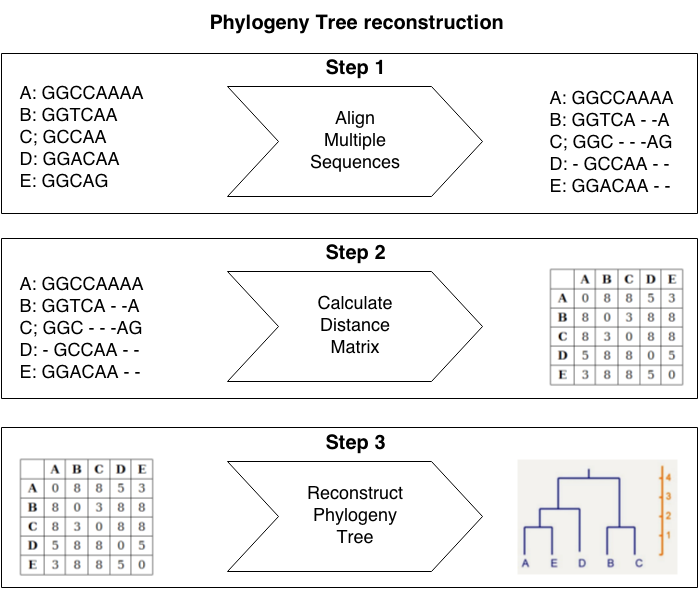
\includegraphics[width=1\textwidth]{reconstructing}
  \caption[w]{Main steps to reconstruct phylogenetic tree.} 
  \label{img:rec1}  
\end{figure}

The next chapter will be devoted to these steps.

\addcontentsline{toc}{section}{\numberline{}Conclusion for Chapter 1}
\section*{Conclusion for Chapter 1}

- Main goal of the phylogeny is to reconstruct 
phylogenetic tree.

- Phylogenetic tree represents evolutionary 
histories of living organisms.

- Algorithms of estimate calculations can be used to
analyze phylogenetic data.
%\subsection{Phase 3} \label{phase3}


\newpage
 
% BOB II
\chapter{State of Art}
\section{Previous Researches}
To show the novelty of my work, at first need to understand what was researched previously.

Same stages of the actions are used to construct a phylogenetic tree in many methods.
They can be divided in three main actions.
It is necessary to align sequences so that able to compare each other. 
One of the earliest formalizations of multiple sequence when it as the 
problem of reconstructing ancient predecessors to contemporary sequences 
when the topology of a tree describing the evolution of the sequences is given.
The edit distances between the sequences at the nodes of this tree define the 
lengths of the edges. The problem is to choose the ancient sequence such that 
the overall length of th tree is minimized. This formulation is called 
``tree-alligment''. It is one of two commonly used formulations of multiple 
sequence alignment, the other one being the so-called sum-of-pairs alignment.

\subsection{Multiple Sequence Alignment}
Alignment methods vary in type of data (DNA, RNA, or amino-acid)
they can handle, and also, to some extent, the objectives of the alignment method \cite{tandy}.
Thus, some methods are designed exclusively for proteins, some exclusively
for RNAs, but many alignment methods can analyze both protein and nucleotide
datasets. We refer to methods that can analyze all types of molecular sequences as
``generic'' methods.

Alignment methods are used to predict function and structure, to determine whether a
sequence belongs to a particular gene family or superfamily, to recognize homology in the
``twilight zone'' (where sequence similarity is so low that homology is dificult to detect),
to infer selection, etc.. On the other hand, alignment methods are also used in order
to estimate a phylogeny. As we shall see, the design of alignment methods and how they
are evaluated depend on the purpose they are being used for.


\subsubsection{MSA Evaluation Criteria}
The standard criteria used to evaluate alignments for
accuracy are based on shared homologies between the true and the estimated alignment,
with the SP-score (sum-of-pairs score) measuring the fraction of the true pairwise
homologies correctly recovered, and the TC-score (``total column'' score) measuring the
number of identical columns. Variants on these criteria include the true metrics suggested
by Blackburne et al. and the consideration of diferent types of alignment error (i.e.,
both false positive and false negative) rather than one overall measure of ``alignment
accuracy''. Other criteria, such as the identification and correct alignment of specific
regions within a protein or rRNA, have also been used. Furthermore, because
sequence alignment has the potential to impact phylogeny estimation, a third way of
evaluating a multiple sequence alignment method is via its impact on phylogeny estimation

\subsubsection{Benchmark datasets}
Many studies have
evaluated MSA methods using biological data for which structurally informed alignments
are available. The best known of these benchmark datasets is probably BAliBASE,
but others are also used. The choice of benchmarks and how they are used
has a large impact on the result of the evaluation, and so has been discussed in several
papers.

From the perspective of phylogeny estimation, one of the
most important of their observations is that structurally-defined benchmarks often omit
the highly variable parts of the molecule, including introns. Thus, an alignment can be
considered completely correct as a structural alignment if it aligns the conserved regions,
even if it fails to correctly align the variable regions. The problem with this criterion (as
they point out) is that the highly variable portions are often the sites that are of most use
for phylogeny estimation, whereas sites that change slowly have little phylogenetic signal.

\subsubsection{Relative performance of MSA methods}
While most studies have evaluated alignment methods in terms of standard criteria 
(notably, SP and TC scores) on biological
benchmarks, some studies have explored alignment estimation for phylogeny estimation
purposes. As commented on earlier, many studies have shown that alignment estimation
impacts phylogenetic estimation, and that alignment and tree error increase with the rate
of evolution. Also, on very large datasets, due to computational limitations, only a few
alignment methods can even be run (and typically not the most accurate ones), which
results in increased alignment error. On the other hand, on large trees with rates of
evolution that are sufficiently low, alignment estimation methods can differ substantially
in terms of SP-score without impacting the accuracy of the phylogenetic tree estimated
using the alignment. More generally, standard alignment metrics may be only poorly
correlated with tree accuracy in some conditions.

\subsubsection{Progressive aligners, and the impact of guide trees}
Many alignment methods
use progressive alignment on a guide tree to estimate the alignment; thus the choice of the
guide tree and its impact on alignment and phylogeny estimation is also of interest. 
Nelesen studied the impact of the guide tree on alignment methods,
and showed that improved phylogenetic accuracy can be obtained by first estimating a tree
from the input using a good two-phase method (RAxML on a MAFFT alignment).
They noted particular benefits in using Probcons with this guide tree, and called the
resultant method ``Probtree''. Prank has also been observed to be very sensitive to guide
trees, and to give improved results by the use of carefully computed guide trees
(maximum likelihood on good alignments). Another study showed that even
when the alignment score doesn't change, the alignment itself can change in important
ways when guide trees are changed. Finally, Capela-Gutierrez and Gabaldon
found that the placement of gaps in an alignment results from the choice of the guide tree,
and hence the gaps are not phylogenetically informative. Based on these observations,
Capela-Gutierrez and Gabaldon recommended that alignment estimation methods should
use the true tree (if possible), or else use an iterative co-estimation method that infers
both the tree and the alignment.

\subsubsection{Template-based methods}
Some alignment methods use a very different type of
algorithmic structure, which is referred to as being ``template-based''. Instead of
using progressive alignment on a guide tree, these methods use models (either profiles,
templates, or Hidden Markov Models) for the gene of interest, and align each sequence to
the model in order to produce the final multiple sequence alignment, as follows. First, a
relatively small set of sequences from the family is assembled, and an alignment estimated
for the set. Then, some kind of model (e.g., a template or a Hidden Markov Model) is
constructed from this ``seed'' alignment. This model can be relatively simple or quite
complex, typically depending on whether the model provides structural information. Once
the model is estimated, the remaining sequences are added to the growing alignment. The
model is used to align each sequence to the seed alignment (which does not change during
the process), and then inserted into the growing alignment. Since the remaining sequences
are only compared to the seed alignment, homologies between the remaining sequences
can only be inferred through their homologies to the seed alignment. Thus, the choice
of sequences in the seed alignment and how it is estimated can have a big impact on
the resultant alignment accuracy. By design, once the seed alignment and the model
are computed, the running time scales linearly with the number of sequences, and the
algorithm is trivially parallelizable. Thus, these methods, which we will refer to jointly as
``template-based methods'', can scale to very large datasets with hundreds of thousands
of sequences.

There are several examples of methods that use this approach. Some of these methods use curated seed alignments based on
structure and function of well-characterized proteins or rRNAs; for example, the protein
alignment method by Neuwald and the rRNA sequence alignment method by Gardner 
use curated alignments. Constraint-based methods, such as COBALT,
3DCoffee and PROMALS, similarly use external information like structure and
function, but then use progressive alignment techniques (or other such methods) to 
produce the final alignment. Clustal-Omega also has a version, called ``External Profile
Alignment'', that uses external information (in the form of alignments) to improve the
alignment step.

Finally, PAGAN is another member of this class of methods; however, it has
some specific methodological differences to the others. First, unlike several of the others,
it does not use external biological information (about structure, function, etc.) to define
its seed alignment. Second, while the others tend to use either HMMs, profiles, or 
templates as a model to define the alignment of the remaining sequences, PAGAN estimates
a tree on its seed alignment, and estimates sequences for the internal nodes. These 
sequences are then used to define the incorporation of the remaining sequences to the seed
alignment. This technique is very similar to the technique used in PaPaRa, which
was developed for the phylogenetic placement problem. Thus, PAGAN
is one of the ``phylogeny-aware'' alignment methods, a technique that is atypical of these
template-based methods, but shared by progressive aligners. PAGAN was compared to an
HMM-based method (using HMMER on the reference alignment to build an HMM, and
then using HMMALIGN to align the sequences to the HMM) on several datasets.
The comparison showed that PAGAN had very good accuracy, better than HMMALIGN,
under low rates of evolution, and that both methods had reduced accuracy under high
rates of evolution. They also noted that PAGAN failed to align some sequences under
model conditions with high rates of evolution, while HMMER aligned all sequences; 
however, the sequences that both HMMER and PAGAN aligned were aligned more accurately
using PAGAN.

\subsubsection{Methods that use divide-and-conquer on the taxon set}
Some alignment methods use a divide-and-conquer strategy in which the 
taxon set is divided into subsets
(rather than the sites) in order to estimate the alignment; these include the 
mega-phylogeny method developed by Smith, SAT'e, SATCHMO-JS,
PROMALS, and the method by Neuwald. (The SAT'e and SATCHMO-JS 
methods co-estimate alignments and trees, and so are not strictly speaking just alignment
methods.) Neuwald's method is a bit of an outlier in this set, because the user provides
the dataset decomposition, but we include it here for comparative purposes.

While the methods differ in some details, they use similar strategies to estimate 
alignments. Most estimate an initial tree, and then use the tree to divide the dataset into
subsets. The method to compute the initial trees differs, with SATCHMO-JS using a
neighbor joining (NJ) tree on a MAFFT alignment, SAT'e using a maximum 
likelihood tree on a MAFFT alignment, PROMALS using a UPGMA tree on $k$-mer distances,
and mega-phylogeny using a reference tree and estimated alignment.

The subsequent division into subsets is performed in two ways. In the case of 
mega-phylogeny, SATCHMO-JS, and PROMALS, the division into subsets is performed by
breaking the starting tree into clades so as to limit the maximum dissimilarity between
pairs of sequences in each set. In contrast, SAT'e-2 removes centroid edges from the
unrooted tree, recursively, until each subset is small enough (below 200 sequences). Thus,
the sets produced by the SAT'e-2 decomposition do not form clades in the tree, unlike the
other decompositions. Furthermore, the sets produced by the SAT'e-2 decomposition are
guaranteed to be small (at most 200 taxa) but are not constrained to have low pairwise
dissimilarities between sequences.

Alignments are then produced on each subset, with PROMALS, SAT'e, and 
mega-phylogeny estimating alignments on each subset, and SATCHMO-JS using the alignment
induced on the subset by the initial MAFFT alignment.

These alignments are then merged together into an alignment on the full set, but the
methods use different techniques. PROMALS and mega-phylogeny use template-based
methods to merge the alignments together, while SATCHMO-JS and SAT'e use progressive
alignment techniques. PROMALS also uses external knowledge about protein structure
to guide the template-based merger of the alignments together. PROMALS, 
SATCHMO-JS, and mega-phylogeny use sophisticated methods to merge subset-alignments, but SAT'e
uses a very simple method (Muscle) to merge subset-alignments.

\subsubsection{Very large-scale alignment}
When the datasets are very large, containing many
thousands of sequences, only a few alignment estimation methods are able to run. As
noted, the template-based methods (including PROMALS and mega-phylogeny) scale
linearly with the number of taxa, and so can be used with very large datasets. SAT'e
and SATCHMO-JS are not quite as scalable; however, SAT'e has been able to analyze
nucleotide datasets with about 28,000 sequences. Other methods that have been shown to
run on very large datasets include Clustal-Omega, MAFFT-PartTree, and 
Kalign-2, but many methods fail to run on datasets with tens of thousands of sequences.
Of these, Clustal-Omega is only designed for protein sequences, but MAFFT-PartTree
and Kalign-2 can analyze both nucleotide and amino-acid sequences.

SAT'e is computationally limited by its use of progressive alignment and maximum
likelihood method (RAxML or FastTree-2) in each iteration; both impact the 
running time and - in the case of large numbers of long sequences - memory usage. However,
although limited to datasets with perhaps only 30,000 sequences (or so), on fast-evolving
datasets with 1000 or more sequences, SAT'e provides improvements in phylogenetic 
accuracy relative to competing methods.

\subsection{Stochastic models of sequence evolution}
We begin with a description of the simplest stochastic models of DNA sequence 
evolution, and then discuss amino-acid sequence evolution models and codon evolution models.
The simplest models of DNA sequence evolution treat the sites within the sequences 
independently. Thus, a model of DNA sequence evolution must describe the probability
distribution of the four states, A, C, T, G, at the root, the evolution of a random site (i.e.,
position within the DNA sequence) and how the evolution differs across the sites. 
Typically the probability distribution at the root is uniform (so that all sequences of a fixed
length are equally likely). The evolution of a single site is modeled through the use of
``stochastic substitution matrices'', $4 x 4$ matrices (one for each tree edge) in which every
row sums to 1. A stochastic model of how a single site evolves can thus have up to 12 free
parameters. The simplest such model is the Jukes-Cantor model, with one free parameter,
and the most complex is the General Markov model, with all 12 parameters:

\begin{defn}
The General Markov (GM) model of single-site evolution is defined as follows.

\begin{enumerate}
	\item The nucleotide in a random site at the root is drawn from a known distribution, in
which each nucleotide has positive probability.
	\item The probability of each site substitution on an edge $e$ of the tree is given by a $4 x 4$
stochastic substitution matrix $M(e)$ in which $det(M(e))$ is not $0$, $1$, or $-1$.	
\end{enumerate}
\end{defn}

This model is generally used in a context where all sites evolve identically and 
indpendently (the i.i.d. assumption), with rates of evolution drawn typically drawn from a
gamma distribution. (Note that the distribution of the rates-across-sites has an impact
on phylogeny estimation and dating, as discussed by Evans and Warnow.) In what
follows, we will address the simplest version of the GM model so that all sites have the
same rate of evolution.

We denote a model tree in the GM model as a pair, ($T, {M(e): e \in E(T)}$), or more
simply as $(T, M)$. For each edge $e \in E(T)$, we define the length of the edge $\lambda(e)$ to
be - $log |det(M(e))|$. This allows us to define the matrix of leaf-to-leaf distances, ${\lambda_{ij}}$,
where $\lambda_{ij} = \sum_{e \in P_{ij}}$
$\lambda(e)$, and where $P_{ij}$ is the path in $T$ between leaves $i$ and $j$. A
matrix defined by path distances in a tree with edge weights is called ``additive'', and it
is a well-known fact that given any additive matrix, it is easy to recover the underlying
leaf-labelled tree T for that matrix in polynomial time.

This general model of site evolution subsumes the great majority of other models
examined in the phylogenetic literature, including the popular General Time Reversible
(GTR) model, which requires only that $M(e) = M(e')$
for all edges $e$ and $e'$. 
Further constraints on the matrix $M(e)$ produce the Hasegawa-Kishino-Yang (HKY) model,
the Kimura 2-parameter model (K2P), the Kimura 3-ST model (K3ST), the Jukes-Cantor
model (JC), etc. These models are all special cases of the General Markov model, because
they place restrictions on the form of the stochastic substitution matrices. The standard
model used for nucleotide phylogeny estimation is GTR+gamma, i.e., the General Time
Reversible (GTR) model of site substitution, equipped with a gamma distribution of rates
across sites.

\subsubsection{Protein models}
Just as with DNA sequence evolution models, there are Markov
models of evolution for amino-acid sequences, and also for coding DNA sequences. These
models are described in the same way - a substitution matrix that governs the tree,
and then branch lengths. While the GTR model can be extended to amino-acids (to
produce a $20x20$ matrix) or to codon-based models (to produce a $64x64$ matrix), both
of which must be estimated from the data, in practice these models use fixed matrices,
each of which was estimated from external biological data. The most well known protein
model is the Dayhoff model, but improved models have been developed in recent
years. Similarly, codon-based models have also been based on fixed $64x64$
matrices. In practice, the selection of a protein model for a given dataset
is often done using a statistical test, such as ProtTest, and then fixed. In the
subsequent tree estimation performed under that model, only the tree and its branch
lengths need to be estimated.

\subsection{Phylogeny Estimation Methods}
There are many different phylogeny estimation methods, too numerous to mention here.
However, the major ones can be classified into the following types:

\begin{itemize}
	\item distance-based methods, which first compute a pairwise distance matrix (usually
based on a statistical model) and then compute the tree from the matrix,
	\item maximum parsimony and its variants, which seek a tree with a total minimum
number of changes (as defined by edit distances between sequences at the endpoints
on the edges of the tree),
	\item maximum likelihood, which seeks the model tree that optimizes likelihood
under the given Markov model, and
	\item Bayesian MCMC methods, which return a distribution on trees rather than a single
tree, and also use likelihood to evaluate a model tree.	
\end{itemize}

\subsection{Statistical Performance Criteria}
We discuss three concepts here: \textit{identifiability, statistical consistency, 
and sequence length requirements}.


\textbf{Identifiability:} A statistical model or one of its parameters is said to be 
``identifiable'' if it is uniquely determined by the probability distribution 
defined by the model. Thus, in the context of phylogeny estimation, the 
unrooted model tree topology is identifiable if it is determined by the 
probability distribution (defined by the model tree, which includes the 
numeric parameters) on the patterns of nucleotides at the leaves of the tree. 
In the case of nucleotide models, the state at each leaf can be A,C,T, or G, 
and so there are $4^n$ possible patterns in a tree with n leaves 
(similarly, there are $20^n$ possible patterns for amino-acid models). 
It is well known that the unrooted tree topology is identifiable under 
the General Markov model, and recent work has extended this to 
other models.

\textbf{Statistical Consistency:} We say that a method $\Phi$ is ``statistically consistent'' 
for estimating the topology of the model tree $(T,\theta )$ if the trees estimated 
by $\Phi$ converges to the unrooted version of $T$ (denoted by $T^u$) as the number 
of sites increases. (Note that under this definition, we are not concerned 
with estimating the numeric parameters.) Equivalently, for all $\varepsilon > 0$ there 
is a sequence length $K$ so that if a set $S$ of sequences of length $k \geq K$ are 
generated by $(T,\theta)$, then the probability that $\Phi(S) = T^u$ is at least $1-\varepsilon$. 
We say that a method is statistically consistent under the GM model if 
it is statistically consistent for all model trees in the GM model. 
Similarly, we say a method is statistically consistent under the GTR 
model if it is statistically consistent under all model trees in the GTR model. 

Many phylogenetic methods are statistically consistent under the GM model, 
and hence also under its submodels (e.g., the GTR model). For example, 
maximum likelihood, neighbor joining (and other distance-based methods) 
for properly computed pairwise ``distances'', and Bayesian MCMC methods, 
are all statistically consistent. Onthe other hand, maximum parsimony and 
maximum compatibility are not statistically consistent under the GM 
model. In addition, it is well known that maximum likelihood can be 
inconsistent if the generative model is different from the model 
assumed by maximum likelihood, but maximum likelihood can even be 
inconsistent when its assumptions match the generative model, 
if the generative model is too complex! For example, 
Tuffey and Steel showed that maximum likelihood is equivalent 
to maximum parsimony under a very general ``no-common-mechanism'' model, 
and so is inconsistent under this model. In this case, the model 
itself is not identifiable, and this is why maximum likelihood 
is not consistent. However, there are identifiable models for 
which ML is not consistent, as observed by Steel.

\textbf{Sequence length requirement:} Clearly, statistical consistency 
under a model is a desirable property. However, statistical consistency 
does not address how well a method will work on finite data. 
Here, we address the ``sequence length requirement'' of a phylogeny 
estimation method $\Phi$, which is the number of sites that $\Phi$ needs 
to return the (unrooted version of the) true tree with 
probability at least $1 - \epsilon$ given sequences that evolve 
down a given model tree $(T,\theta)$. Clearly, the number of 
sites that suffces for accuracy with probability at 
least $1 - \epsilon$ will depend on $\Phi$ and $\epsilon$, but it also 
depends on both $T$ and $\theta$. 

We describe this concept in terms of the Jukes-Cantor model, 
since this is the simplest of the DNA sequence evolution models, 
and the ideas are easiest to understand for this model. However, 
the same concepts can be applied to the more general models, and 
the theoretical results that have been established regarding sequence 
length requirements extend to the GM (General Markov) model, which 
contains the GTR model and all its submodels.

In the Jukes-Cantor (JC) model, all substitutions are equally likely, 
and all nucleotides have equal probability for the root state. 
Thus, a Jukes-Cantor model tree is completely defined by the rooted 
tree $T$ and the branch lengths $\lambda(e)$, where $\lambda(e)$ is 
the expected number of changes for a random site on the edge $e$. 
It is intuitively obvious that as the minimum branch length 
shrinks, the number of sites that are needed to reconstruct the 
tree will grow, since a branch on which no changes occur 
cannot be recovered with high probability (the branch will appear 
in an estimated tree with probability at most one-third, 
since at best it can result from a random resolution of a 
node of degree at least 4). It is also intuitively obvious 
that as the maximum branch length increases, the number of 
sites that are needed will increase, since the two sides 
of the long branch will seem random with respect to each other. 
Thus, the sequence length requirement for a given method to be 
accurate with probability at least $1 - \epsilon$ will be 
impacted by the shortest branch length f and the longest 
branch length $g$. It is also intuitively obvious that the 
sequence length requirement will depend on the number of 
taxa in the tree.  

Expressing the sequence length requirement for the 
method $\Phi$ as a function of these parameters ($f,g,n$ and $\epsilon$) 
enables a different - and finer - evaluation of the method's performance 
guarantees under the statistical model. Hence, we consider $f,g$, and $\epsilon$ 
as fixed but arbitrary, and we let JCf,g denote all Jukes-Cantor model 
trees with $0 < f \leq \lambda(e) \leq g < \infty$ for all edges $e$. 
This lets us bound the sequence length requirement of a method as a 
function only of $n$, the number of leaves in the tree. 

The definition of ``absolute fast convergence'' under the Jukes-Cantor 
model is formu- lated as an upper bound on the sequence length requirement, 
as follows:

\begin{defn}
A phylogenetic reconstruction method $\Phi$ is absolute fast-converging (afc) 
for the Jukes-Cantor (JC) model if, for all positive $f,g$, and $\varepsilon$, 
there is a polynomial $p(n)$ such that, for all $(T,\theta)$ in $JC_{f,g}$, 
on set $S$ of $n$ sequences of length at least $p(n)$ generated on $T$, 
we have $Pr[\Phi(S) = T^u] > 1 - \varepsilon$.
\end{defn}

Note also that this statement only refers to the estimation of the unrooted 
tree topology $T^u$ and not the numeric parameters $\Phi$. Also, note that 
the method $\Phi$ operates without any knowledge of parameters $f$ or $g$-or 
indeed any function of $f$ and $g$. Thus, although the polynomial $p$ 
depends upon both $f$ and $g$, the method itself will not. Finally, this 
is an upper bound on the sequence length requirement, and the actual 
sequence length requirement could be much lower. 

The function $p(n)$ can be replaced by a function $f(n)$ that is not 
polynomial to provide an upper bound on the sequence length requirement 
for methods that are not proven to be absolute fast converging. 

\subsection{Empirical Performance}
So far, these discussions have focused on theoretical guarantees under a model, 
and have addressed whether a method will converge to the true tree given 
long enough sequences (i.e., statistical consistency), and if so, then 
how long the sequences need to be (sequence length requirements). However, 
these issues are purely theoretical, and do not address how accurate the 
trees estimated by methods are in practice (i.e., on data). In addition, 
the computational performance (time and memory usage) of phylogeny estimation 
methods is also important, since a method that is highly accurate but will 
use several years of compute time will not generally be useful in most analyses. 

Phylogenetic tree accuracy can be computed in various ways, and there are 
substantive debates on the ``right'' way to calculate accuracy; however, 
although disputed, the Robinson-Foulds (RF) distance, also called the 
``bipartition distance'', is the most commonly used metric on phylogenetic trees. 
We describe this metric here. 

Given a phylogenetic tree $T$ on $n$ taxa, each edge can be associated 
with the bipartition it induces on the leaf set; hence, the tree 
itself can be identified with the set of leaf- bipartitions defined 
by the edges in the tree. Therefore, two trees on the same set 
of taxa can be compared with respect to their bipartition sets. 
The RF distance between two trees is the size of the symmetric difference 
of these two sets, i.e., it is the number of bipartitions that are in one 
tree's dataset but not both. This number can be divided by $2(n - 3)$ 
(where n is the number of taxa) to obtain the ``RF rate''. In the context 
of evaluating phylogeny estimation methods, the RF distance is sometimes 
divided into false negatives and false positives, where the false 
negatives (also called ``missing branches'') are branches in the 
true tree that are not present in the estimated tree, and the 
false positives are the branches in the estimated tree that are not 
present in the true tree. This distinction between false positives 
and false negatives enables a more detailed comparison between trees 
that are not binary.

Many studies have evaluated phylogeny estimation methods on simulated 
data, varying the rate of evolution, the branch lengths, the number 
of sites, etc. These studies have been enormously informative about 
the differences between methods, and have helped biologists make 
informed decisions regarding methods for their phylogenetic analyses. 
Some of the early simulation studies explored performance on very 
small trees, including the fairly exhaustive study by Huelsenbeck 
and Hillis on 4-leaf trees, but studies since then have explored 
larger datasets and more complex questions. For example, studies 
have explored the impact of taxon sampling on phylogenetic 
inference, the impact of missing data on phylogenetic inference, 
and the number of sites needed for accuracy with high probability. 
In fact, simulation studies have become, perhaps, the main way to 
explore phylogenetic estimation. 

\subsubsection{Distance-based methods} \label{methods}
Distance-based methods operate by first computing a matrix of 
distances (typically using a statistically defined technique, 
to correct for unseen changes) between every pair of sequences, 
and then construct the tree based on this matrix. Most, but not all, 
distance-based methods are statistically consistent, and so will 
be correct with high probability, given long enough sequences. 
In general, distance-based methods are polynomial time, and so 
have been popular for large-scale phylogeny estimation. 
While the best known distance-based method is probably neighbor 
joining, there are many others, and many are faster and/or 
more accurate. 

One of the interesting properties about distance-based 
methods is that although they are typically guaranteed 
to be statistically consistent, not all distance-based 
methods have good empirical performance! A prime example 
of this lesson is the Naive Quartet Method, a method that 
estimates a tree for every set of four leaves using the 
Four-Point Method (a statistically-consistent distance method) 
and then returns the tree that is consistent with all the 
quartets if it exists. It is easy to show that the Naive 
Quartet Method runs in polynomial time and is statistically 
consistent under the General Markov model; however, because 
it requires that every quartet be accurately estimated, 
it has terrible empirical performance! Thus, while 
statistical consistency is desirable, in many cases statistically 
inconsistent methods can outperform consistent ones.

\subsubsection{Maximum parsimony}
Maximum parsimony (MP) is NP-hard, and so the methods for 
MP use heuristics (most without any performance guarantees). 
The most efficient and accurate maximum parsimony software 
for very large datasets is probably TNT, but PAUP* is also 
popular and effective on datasets that are not extremely large. 
TNT is a particularly effective parsimony heuristic for 
large trees, and has been able to analyze a multi-marker 
sequence dataset with more than 73,000 sequences.

\subsubsection{Maximum likelihood}
Maximum likelihood (ML) is also NP-hard, and so attempts to 
solve ML are also made using heuristics. While the heuristics 
for MP used to be computationally more efficient than the 
heuristics for ML, the current set of methods for ML are 
quite effective at ``solving'' large datasets. (Here the 
quotes indicate that there is no guarantee, but reasonably 
good results do seem to be obtained using the current best software.)

The leading methods for large-scale ML estimation under the 
GTR+Gamma model include RAxML, FastTree-2, PhyML, and GARLI. 
Of these four methods, RAxML is clearly the most frequently 
used ML method, in part because of its excellent parallel 
implementations. However, a recent study showed that trees 
estimated by FastTree-2 were almost as accurate as those 
estimated by RAxML, and that FastTree-2 finished in a 
fraction of the time; for example, FastTree-2 was able to 
analyze an alignment with almost 28,000 rRNA sequences 
in about 5 hours, but RAxML took much longer. 
Furthermore, FastTree-2 has been used to analyze larger 
datasets (ones with more sequences) than RAxML: the 
largest dataset published with a RAxML analysis 
had 55,000 nucleotide sequences, but FastTree has 
analyzed larger datasets. For example, FastTree-2 
has analyzed a dataset with more than 1 million nucleotide 
sequences, and another with 330,556 sequences. 
The reported running time for these analyses are 203 
hours for the million-taxon dataset, and 13 hours 
(with 4 threads) for the 330K- taxon dataset 
\footnote{Morgan Price, personal communication, May 1, 2013.}. 
By comparison, the RAxML analysis of 55,000 nucleotide 
sequences took between 100,000 and 300,000 CPU hours
\footnote{Alexis Stamatakis, personal communication, May 1, 2013.}. 
The difference in running time is substantial, but we 
should note two things: the RAxML analysis was a 
multi-marker analysis, and so the sequences were much 
longer (which impacts running time), and because RAxML 
is highly parallelized, the impact of the increased running 
time is not as significant (if one has enough processors). 
Nevertheless, for maximum likelihood analysis of alignments 
with large numbers of sequences, FastTree-2 provides 
distinct speed advantages over RAxML.  

There are a few important limitations for FastTree-2, 
compared to RAxML. First, FastTree-2 obtains its speed by 
somewhat reducing the accuracy of the search; thus, the 
trees returned by FastTree-2 may not produce maximum 
likelihood scores that are quite as good as those produced 
by RAxML. Second, FastTree-2 doesn't handle very long 
alignments with hundreds of thousands of sites very well, 
while RAxML has a new implementation that is designed 
specifically for long alignments. Third, FastTree-2 has a 
smaller set of models for amino-acid analyses than RAxML. 
Therefore, in some cases (e.g., for wide alignments, 
and perhaps for amino-acid alignments), RAxML may 
be the preferred method. 

However, the ML methods discussed above estimate trees under 
the GTR+Gamma model, which has simplifying assumptions that 
are known to be violated in biological data. 
The nhPhyml method is a maximum likelihood method for 
estimating trees under the non-stationary, non-homogeneous 
model of Galtier and Guoy, and hence provides an 
analytical advantage in that it can be robust to some 
violations of the GTR+Gamma model assumptions. However, 
nhPhyml seems to be able to give reliably good analyses 
only on relatively small datasets (i.e., with at most a 
few hundred sequences, or fewer sequences if they are very long). 
The explanation is computational - it uses NNI 
(nearest neighbor interchanges, see below) to search treespace, 
but NNI is relatively ineffective, which means that it is 
likely to get stuck in local optima. This is unfortunate, 
since large datasets spanning substantial evolutionary 
distances are most likely to exhibit an increased incidence 
in model violations. Therefore, highly accurate phylogeny 
estimation of large datasets may require the use of new 
methods that are based upon more realistic, and more general, 
models of sequence evolution.

\subsubsection{Bayesian MCMC methods}
Bayesian methods are similar to maximum likelihood methods 
in that the likelihood of a model tree with respect to the 
input sequence alignment is computed during the analysis; 
the main difference is that maximum likelihood selects the 
model tree (both topology and numeric parameters) that 
optimizes the likelihood, while a Bayesian method outputs a 
distribution on trees. However, once the distribution is 
computed, it can be used to compute a single point estimate 
of the true tree using various techniques (e.g., a consensus 
tree can be computed, or the model tree topology with the 
maximum total probability can be returned).

The standard technique used to estimate this distribution 
is a random walk through the model tree space, and the 
distribution is produced after the walk has converged to 
the stationary distribution.

There are many different Bayesian methods (e.g., MrBayes, BEAST, 
PhyloBayes, p4, and BayesPhylogenies), differing in terms 
of the techniques used to perform the random walk, and 
the model under which the likelihood is computed; however, 
MrBayes is the most popular of the methods. Bayesian 
methods provide theoretical advantages compared to 
maximum likelihood methods. However, the proper use of a 
Bayesian MCMC method requires that it run to convergence, 
and this can take a very long time on large datasets. 
Thus, from a purely empirical stand- point, Bayesian 
methods do not yet have the scalability of the best 
maximum likelihood methods, and they are generally 
not used on very large datasets.

\subsubsection{Comparisons between methods}
Simulation studies have shown some interesting 
differences between methods. For example, the 
comparison between neighbor joining and maximum 
parsimony reveals that the relative performance may 
depend on the number of taxa and the rate of evolution, 
with maximum parsimony sometimes performing better 
on large trees with high rates of evolution, even 
though the reverse generally holds for smaller trees.  

More generally, most simulation studies have shown 
that maximum likelihood and Bayesian methods 
(when they can be run properly) outperform maximum 
parsimony and distance-based methods in many 
biologically realistic conditions 
(see Wang et al. for one such study).

\subsubsection{Heuristics for exploring treespace}
Since both maximum likelihood and maximum parsimony 
are NP-hard, methods for ``solving'' these problems 
use heuristics to explore the space of different tree 
topologies. These heuristics differ by the techniques 
they use to score a candidate tree (with the best 
ones typically using information from previous 
trees that have already been scored), and how 
they move within treespace. 
 
% \section{Methods of research}
\section{Benefit for the Science}
\newpage

% BOB III
\chapter{Design and Implementation}
\section{Solution for given problem}
\section{The research results}

\newpage

\chapter*{Conclusion}
\addcontentsline{toc}{chapter}{\numberline{}Conclusion}
This chapter set out to survey large-scale phylogeny and alignment estimation. 
As we have seen, large-scale alignment and phylogeny estimation 
(whether of species or of individual genes) is a complicated problem. 
Despite the multitude of methods for each step, the estimation of very 
large sequence alignments or gene trees is still quite diffcult, 
and the estimation of species phylogenies (whether trees or networks!), 
even more so. Furthermore, the challenges in large-scale estimation 
are not computational feasibility (running time and memory), as 
inferential methods can differ in their theoretical and empirical 
performance. 

\newpage

\nocite{*} 

% \clearpage
%%\addcontentsline{toc}{chapter}{\bibname}

%\bibliographystyle{plainnat}	
%\bibliography{biblio}
% \settocbibname{References} 
\renewcommand{\bibname}{References}
\addcontentsline{toc}{chapter}{\numberline{}References}
\bibliographystyle{plainnat}	
\bibliography{biblio}

% \begin{appendices}
% 
% The contents...
% asdasdas
% \end{appendices}
\clearpage

% \addcontentsline{toc}{chapter}{\numberline{}Appendices}
% \appendix
% \section*{Appendices}
\addcontentsline{toc}{chapter}{\numberline{}Appendices}
\appendix
\section*{Appendices}

% \lstinputlisting[language=java]{TestFastaReader.java}
\lstinputlisting[language=java]{PhyloUI.java}
\lstinputlisting[language=xml]{full.xml}






\end{document}